\documentclass[11pt,twocolumn,DIV=11]{scrartcl}

\usepackage{amsmath}
\usepackage{framed}
\usepackage{color}
\definecolor{shadecolor}{gray}{0.8}

\usepackage{natbib}
\bibliographystyle{apalike}

\usepackage{tikz}
\usetikzlibrary{bayesnet}

\renewcommand\phi\varphi
\DeclareMathOperator*{\argmax}{arg\,max}

\author{
    Verdegaal, Jacob\\
    \texttt{jacob.verdegaal@student.uva.nl}
    \and
    Drumm, Eli\\
    \texttt{etd@dte.li}
    \and
    Noble, Bill\\
    \texttt{winobes@gmail.com}
}

\title{Inducing Semantic Frames on a Very Large Corpus of Syntactic-Ngrams}

\begin{document}

\maketitle


\section{Introduction}
Here we provide some background information about what are semantic frames and 
what it menas to induce them and stuff like that.


\section{Related Work}
Here we talk mostly about the O'Connor paper \citep{oconnor2013} and the Rooth 
paper \citep{rooth1999}.


\section{Induction Models}

We consider two probabalistic latent-variable models that learn semantic frames
from verb-subject-object tripples (VSO's).
The goal of these models is to use th syntactic information give by a VSO to
infer what kind of event it describes (i.e., to which semantic frame it belongs).

\subsection{Model 0}

The approach models each VSO independenly, without considering any further context.
Word distributions are completely independent between arguments and accross frames.
Tuples are clustered according to which frame's three distributions best fit the 
three arguments.

\begin{figure}[h]

    \begin{snugshade}
    \scriptsize
    For each $i = 1..N$:\\
    \hspace*{15pt} Draw a frame $f \sim \theta$.\\
    \hspace*{15pt} Draw a verb $v \sim \phi_f^v$\\
    \hspace*{15pt} Draw a subject $s \sim \phi_f^s$\\
    \hspace*{15pt} Draw an object $o \sim \phi_f^o$
    \end{snugshade}

    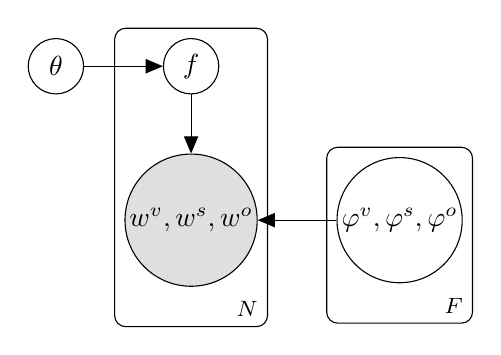
\begin{tikzpicture}
  % Nodes
  \node[obs] (datapoint) {$w^v,w^s,w^o$} ; %
  \node[latent, above=0.75cm of datapoint] (F) {$f$} ; %
  \node[latent, left=of F] (theta) {$\theta$}; %
  \node[latent, right=of datapoint] (phi) {$\varphi^v,\varphi^s,\varphi^o$}; %
  \edge {theta} {F} ; %
  \edge {F} {datapoint}
  \edge {phi} {datapoint} ; %
  \plate {tuples} {(F) (datapoint) } {$N$}; %
  \plate {} {(phi)} {$F$} ; %
\end{tikzpicture}


    \label{gen0}
    \caption{Model 0 generative story}

\end{figure}

Model 0 is based on one originally proposed in \citet{rooth1999}, which 
considers noun-verb pairs. Following \citet{oconnor2013}, we expand the model
to use the limited syntax of VSOs.

The generative story (fig. \ref{gen0}) gives us the following joint probability:
\begin{align*}
&P(\mathbf{f},\mathbf{w}|\phi,\theta) 
  = P(\mathbf{f}|\theta)P(\mathbf{w}|\phi)\\
  =& \prod_{i=1}^{N}\big[\theta(f_i) \prod_a^{\{v,s,o\}}\phi_{f_i}^a(w_i^a)\big]
\end{align*}

Therefore, the incomplete log-likelihood (i.e., where the sequence of frames
is hidden) that we want to maximize is as follows:
\[
L(\theta,\phi) = \sum_{i=1}^N\big[\log \sum_{f_i=1}^F\theta(f_i)\prod_{a}^{\{v,s,o\}}\phi_{f_i}^a(w^a_i)\big]
\]

Expectation maximization can be used to maximize this likelihood.
First we use the current estimates for $\theta$ and $\phi$ to infer a 
distribution over possible choices of frame. This is the E-step. 

\begin{align}
\mu_i(f) =& P(f_i=f, w_i|\phi,\theta)\nonumber\\
=& \frac{\theta(f)\prod_a^{\{v,s,o\}}\phi_f^a(w^a_i)}
                {\sum_{f'=1}^F\theta(f)\prod_a^{\{v,s,o\}}\phi_f^a(w^a_i)}\label{E}
\end{align}

Then in the M-step, we find $\theta$ and $\phi$ that maximize the expectation of
the complete likelihood. In particular, we want to maximize

\begin{align*}
&E_\mu\big[\sum_{i=1}^N\log P(w_i,f_i|\theta,\phi) =\\
=& \sum_{i=1}^N\sum_{f=1}^F\mu_i(f)\log\Big[\theta(f)\prod_a^{\{v,s,o\}}\phi_f^a(w_i^a)\Big]\\
=& \sum_{i=1}^N\sum_{f=1}^F\mu_i(f)\log\theta(f)\\
+& \sum_a^{\{v,s,o\}} \sum_{i=1}^N\sum_{f=1}^F\mu_i(f)\log \phi_f^a(w_i^a)
\end{align*}

Thus the problem is reduced to maximizing each of the terms in the sum above. Fortunately
these have closed for solutions using lagrangian multipliers.


\begin{align}
&\argmax_{\theta(f)}\sum_{i=1}^N\sum_{f=1}^F\mu_i(f)\log\theta(f)\nonumber\\
&= \frac{\sum_{i=1}^N\mu_i(f)}{\sum_{f'}^F\sum_{i=1}^N\mu_i(f)}
\end{align}

and

\begin{align}
&\argmax_{\phi^a(w)}\sum_{i=1}^N\sum_{f=1}^F\mu_i(f)\log \phi_f^a(w_i,a)\nonumber\\
&= \frac{\sum_{i=1}^N \mu_i(f)\,c(w^a)}{\sum_{w'=1}^{V^a}\sum_{i=1}^N \mu_i(f)\,c(w',a)}
\end{align}

Where $c(w,a)$ indicates the number of times word $w$ is observed as argument $a$.

\subsection{Model 1}

As we know from topic modeling, it is the nature of documents that they contain 
sentences with related semantic content. Therefore, it is reasonable to assume 
that semantic frames are not uniformly distributed within documents. Taking 
advantage of this assumption, we can break drop model 0's assumption of independence 
between tuples.

\begin{figure}

    \begin{snugshade}
    \scriptsize
    For each frame $f=1..F$:\\
    \hspace*{15pt} For each argument $a\in\{v,s,o\}$:\\
    \hspace*{30pt} Draw a distribution $\phi_f^a\sim Dirichlet(\beta)$\\
    For each document $d=1..D$:\\
    \hspace*{15pt} Draw a distrbution $\theta_d \sim Dirichlet(\alpha)$\\
    \hspace*{30pt} For each $i = 1..N^d$:\\
    \hspace*{30pt} Draw a frame $f \sim \theta^d$.\\
    \hspace*{30pt} Draw a verb $v \sim \phi_f^v$\\
    \hspace*{30pt} Draw a subject $s \sim \phi_f^s$\\
    \hspace*{30pt} Draw an object $o \sim \phi_f^o$
    \end{snugshade}

    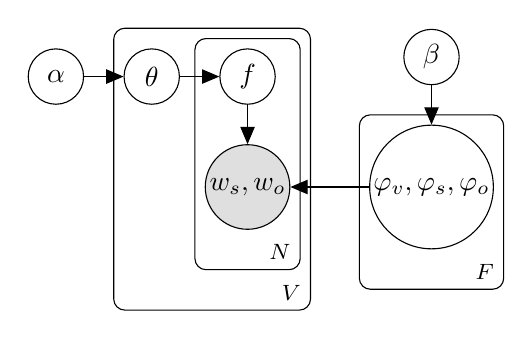
\begin{tikzpicture}[]
    \node[obs]                   (w)     {$w_s,w_o$}; %
    \node[latent, above=0.5cm of w]     (f)     {$f$};
    \node[latent, left=0.5cm of f]     (theta) {$\theta$};
    \node[latent, left=0.5cm of theta] (alpha) {$\alpha$};
    \node[latent, right=of w]    (phi)   {$\varphi_v,\varphi_s,\varphi_o$};
    \node[latent, above=0.5cm of phi] (beta) {$\beta$};
    \edge {alpha} {theta};
    \edge {theta} {f};
    \edge {f} {w};
    \edge {phi} {w};
    \edge {beta} {phi};
    \plate {frames} {(phi)} {$F$};
    \plate {datapoints} {(f) (w)} {$N$};
    \plate {verbs} {(f) (w) (datapoints) (theta)} {$V$};
\end{tikzpicture}


    \caption{Model 1 generative story}

\end{figure}

The independence assumptions int the generative story for model 1 give us the 
following joint distribution:

\begin{align*}
&P(\mathbf{w},\mathbf{f}|\theta,\phi,\alpha,\beta)\\
&=P(\mathbf{w}|\mathbf{f},\phi)\,P(\mathbf{f}|\theta)\,P(\theta|\alpha)\,P(\phi|\beta)
\end{align*}

We can find the marginal distribution of the latent and observed variables by
integrating over the priors:

\begin{align*}
& P(\mathbf{w},\mathbf{f}|\alpha,\beta)\\
&=\int_\phi\int_\theta P(\mathbf{w},\mathbf{f}|\theta,\phi,\alpha,\beta)\\
&=     \int_\phi P(\mathbf{w}|\mathbf{f},\phi )\,P(\phi|\beta)
\times \int_\theta P(\mathbf{f}|\theta)\,P(\theta|\alpha)
\end{align*}


\begin{align}
&p(z_{ij} = f| \mathbf{f}_{-ij},\alpha,\beta,\mathbf{w})\\
&\propto \prod_a^{\{v,s,o\}}\frac{\beta^a + \tilde{c}(f,w_{ij})}{V^a + \tilde{c}(f)}
        \cdot \frac{\alpha + \tilde{c}(i,f)}{f\alpha+\tilde{c}(i)}
\end{align}


\section{Data}

\subsection{Google Syntactic-ngrams}
Here we talk a bit about the syntactic n-grams and all that \citep{ngrams2013}.
\begin{itemize}
    \item A syntactic-ngram is a $k$-word rooted subtree for some sentence. 
    \item Google ngrams come from a corpus of 3.5 million English books.
    \item We trimmed the ``verb args'' dataset to consider only subject-verb-object triples (VSO's).
    \item The dataset contains 1,629,120 unique VSO's with a total of 96,245,401 by count.
    \item In our final results we may only use the most common \%20 of these...
\end{itemize}

\subsection{Pruning}


\section{Experiments}


\section{Results}
\subsection{Frame Coherency}
rame coherency: for a datapoint $(v,s,o)$ and a tuple $(v^r,s,o)$ where $v^r$ is a random choses verb: $P(v\mid s,o) \geq P(v^r\mid s,o)$  
\subsection{Frame Correctness}
Frame correctness: for the top 25 most probable verbs per frame $TV$ and framenet classes of verbs $FN$: \[\frac{2|TV\cap FN|}{|TV|+|FN|}\]
\subsection{Model 0}
\subsection{Model 1}


\section{Discussion}


\section{Future Work}
\begin{itemize}
\item Come up with models that are specifically for independent tuples.
\item Use more of the arguments in verbargs.
\item Use year information -- do frames change over time?
\item Consider subjet/object pairs instead of independent.
\end{itemize}

\section{Conclusion}


\bibliography{refs.bib}
\end{document}
